\documentclass[paper=a4,fontsize=11pt]{article}
\usepackage{amsmath,amssymb,amsthm}
\usepackage[protrusion=true,expansion=true]{microtype}	
\usepackage{algorithm}
\usepackage{algpseudocode}
\usepackage[margin=1.5in]{geometry}
\usepackage{graphicx}
\setlength{\textfloatsep}{0.1cm}
\setlength{\floatsep}{0.1cm}

\begin{document}
\title{TCSS 343 - Assignment 2}
\author{Jake McKenzie}
\maketitle
\begin{enumerate}
\item [(3 points) 1.] Below is a self-reduction for the \texttt{MAX} problem. State a recursive algorithm using pseudocode for finding the maximum element based on this self-reduction.\\
\begin{algorithm}
\caption{Find Max integer in an Array with simple recursion}
\label{array-max}
\begin{algorithmic}[1]
\Procedure{Find Max}{$A$}
    \If{($a == b$)}
        \State return A[a]
    \ElsIf{($a < b$)}
        \State return Max(A[a],Find Max(A[a + 1]))
    \EndIf
\EndProcedure
\Procedure{Max}{$a,b$}
    return ($a < b$) ? b : a
\EndProcedure
\end{algorithmic}
\end{algorithm}
\item [(6 points) 2.] Using the same reduction as part 1 now state a recurrence $T(n)$ that expresses the worst case run time of the recursive algorithm. Find a similar recurrence in your notes and state the tight bound on $T(n)$.\\\\\
Line 3 makes $1$ amount of operations while line 5 makes $T(n-1)$, this is because there are $n-1$ amount of comparisons to check for the max in the recurrence for when this list is greater than 1. **Note**: Consistency of whether the constant amount of operations is writen as $1$ or $O(1)$ are inconsistent so I went with the notation I've seen the most used often.
\[
  T(n) =
    \begin{cases}
        1 & \text{if $n = 1$} \\
        T(n-1) + 1 & \text{if $n > 1$}
    \end{cases}
\]
Claim: $\forall n > 0$, the running time of \textit{Find Max} $\epsilon O(n)$. We consder the recurrance relation above.
\begin{enumerate}
\item[1.] Base Case:\\
$$n = 1; T(1) = 1$$
\item[2.] Inductive Hypothesis:\\
\[
  T(k) =
    \begin{cases}
        1 & \text{if $k = 1$} \\
        T(k-1) + 1 & \text{if $k > 1$}
    \end{cases}
\]
\\Assume for an arbitrary $k, T(k) \leq k$
\item[3.] Inductive Step:
\begin{gather*}
\text{if $k > 1$}\\
T(k + 1) = T(k) + 1\\
T(k + 1) = T(k - 1) + 1 + 1\\  
T(k + 1) = k + 2\\
T(k + 1) \epsilon O(k)\\
\therefore\\
T(k) \epsilon O(k)\\
\end{gather*}
\end{enumerate}
\item [(9 points) 3.] Below is a self-reduction for the \texttt{MAX} problem. State a recursive algorithm using pseudocode for finding the maximum element based on this self-reduction.\\\\\
\[
M(A[a\dots b]) = \left\{
\begin{array}{cl}
-\infty & \textrm{ if } a > b\\
A[a] & \textrm{ if } a = b\\
\max(M(A[a\dots t_1]), \max(M(A[t_1+1\dots t_2]), M(A[t_2+1\dots b]))) & \textrm{ if } a < b
\end{array}
\right.
\]
\begin{algorithm}
\caption{Find Max integer in an Array with 3-Way Split}
\label{array-max}
\begin{algorithmic}[1]
\Procedure{Find Max}{$A,a,t_1,t_2$}
    \If{($a > b$)}
        \State return 0x7FFFFFFF
    \ElsIf{($a == b$)}
        \State return A[a]
    \ElsIf{($a < b$)}
        \State return Max(FindMax(A,a+1,$t_1$,$t_2$), Max(FindMax(A, a, $t_1$+1,$t_2$), FindMax(A, a, $t_1$,$t_2$+1]))
    \EndIf
\EndProcedure
\Procedure{Max}{$a,b$}
    return (a $<$ b) ? b : a
\EndProcedure
\end{algorithmic}
\end{algorithm}\\
For what it's worth, I don't think this algorithm will find the max element if it is contained within the first third of the array(we never iterate over the first third elements, only the second and last third), but it does match the self-reduction.
\item [(7 points) 4.] Using the same reduction as part 3 now state a recurrence $T(n)$ that expresses the worst case run time of the recursive algorithm. You do not need to formally prove your recurrence, but you have to show that it is a reasonable guess by using a recursion tree or by the repeated substitution method.
\textit{Hint: assume that $n$ is a power of 3}.\\\\
I assumed, for purposes of the problem, that we did iterate through each third of the array evenly and like you said that $n = 3^\psi$. Intuitively I expect this to be a worst case linear runtime, which case each last element of the subarrays would be a local max but let propose a semi-formal argument for such. Let us assume the following recurrence reduction.
\[
  T(n) =
    \begin{cases}
        1 & \text{if $n = 1$} \\
        3T(\frac{n}{3}) + d & \text{if $k > 1$}
    \end{cases}
\]
\begin{align*}
\text{if $k > 1$ and $let n = 3^\psi$}\\
T(n) &= 3T(\frac{n}{3}) + d\\
T(n) &= 3T(3^{\psi - 1}) + 3^{\psi} + d\\
T(n) &= 3T(3^{\psi - 2}) + 3^{\psi - 1} + 3^{\psi} + d\\
T(n) &= 3T(3^{\psi - 3}) + 3^{\psi - 2} + 3^{\psi - 1} + 3^{\psi}  + d\\
&\vdots\\
T(n) &= 3^{0} + \dots + 3^{\psi - 2} + 3^{\psi - 1} + 3^{\psi}  + d\\
T(n) &= \sum_{\psi=0}^{k}3^{\psi} + d\\
T(n) &= \frac{3^{k+1} - 1}{2} + d\\
T(n) &= \frac{3n - 1}{2} + d\\
T(n) &= \epsilon O(n)\\
\end{align*}\\
\end{enumerate}
\begin{enumerate}
\item [(12 points) 1.] State two different self-reductions for the \texttt{SUM} problem. Use the self-reduction examples from the lectures as a guide.\\
\\For this problem I decided to use divide and conquer for the second self-reduction and just normal recursion for the second. I don't think these are good ways to sum over an array, there are a lot of wasted computations but it is quite readable. The first algorithm simply completes a summation on the array in reverse order. The second algorithm sums the even and odd elements at the same time.{
\[
  T(n) =
    \begin{cases}
        1 & \text{if $n = 1$} \\
        T(n - 1) + 1 & \text{if $k > 1$}
    \end{cases}
\]
\[
  T(n) =
    \begin{cases}
        1 & \text{if $n = 1$} \\
        2T(n-2) + 1 & \text{if $k > 1$}
    \end{cases}
\]
}
\\\item [(12 points) 2.]{ Give recursive algorithms based on your divide-and-conquer self-reductions to solve the \texttt{SUM} problem.\\\\
\begin{algorithm}
\caption{Find Sum of an Array via Simple Recursion}
\label{array-sum}
\begin{algorithmic}[1]
\Procedure{Find Sum}{$A,n$}
    \If{($n \leq 0$)}
        \State return 0
    \Else
        \State return FindSum(A, n - 1) + A[n - 1]
    \EndIf
\EndProcedure
\end{algorithmic}
\end{algorithm}

\begin{algorithm}
\caption{Find Sum of an Array via Divide and Conquer}
\label{array-sum}
\begin{algorithmic}[1]
\Procedure{Find Sum}{$A,n$}
    \If{($n \leq 0$)}
        \State return 0
    \Else
        \State return FindSum(A, n - 2) + A[n - 1] + A[n - 2] 
    \EndIf
\EndProcedure
\end{algorithmic}
\end{algorithm}
}
\item [(6 points) 3.] What are the worst-case runtimes of the solutions you have generated. (Just state the runtimes. You do not need to show your work.)\\\\
Both algorithm operate in linear time with a worst case runtime of $O(n)$. In fact I can make the argument that both functions are $\Theta(n)$. I came to this conclusion from reading Tim Roughgarden's Algorithms Illuminated page 56-57 where he states then proves theorem $max\{f(n),g(n)\} = \Theta(f(n) + g(n))$. Both algorithms are bounded by some constant multiple of $n$, while algorithm 4 operates slightly slower than 3, they both follow this fact. If we take the max of the two, which would be algorithm 4, that still operates in linear time. From this information I came to the firm conclusion that both algorithms were operating in $\Theta(n)$. I hope this makes sense to you. I know it's a roundabout way of thinking about this problem but it's what helped me come to a conclusion so I thought I would include it.\\\\
Consider the following recurrence $T(n)$:

\[
T(n) = \left\{
\begin{array}{cl}
c & \textrm{ if } n = 1\\
2T(\left\lfloor\frac{n}{4}\right\rfloor) + 16 & \textrm{ if } n > 1
\end{array}
\right.
\]

\begin{enumerate}
\item [(10 points) 1.] Use the recursion tree or repeated substitution method to come up with a good guess for a bound $g (n)$ on the recurrence $T (n)$.\\\\
Consider the following $2T(\left\lfloor\frac{n}{4}\right\rfloor) + 16 \leq 2T(\frac{n}{4}) + 16$ which is always true. From my readings, floor functions are ignored for the conveince of proofs until they matter. I don't like doing that but I don't see any other way to prove this.
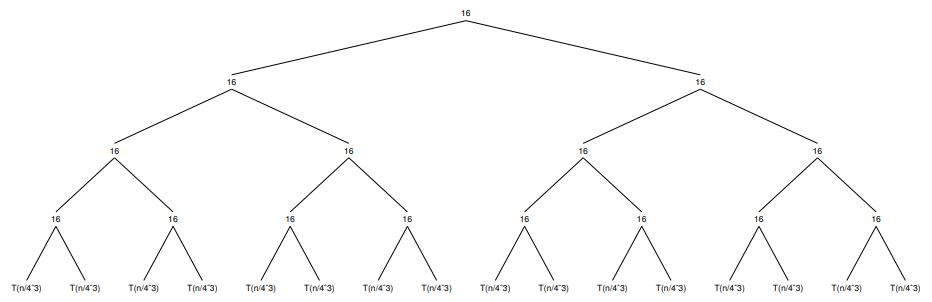
\includegraphics[scale = .5]{tree}\\
This is the recursion tree I obtained. Let the depth of the tree be $\nabla$ and number of nodes be unknown for now, by looking at the tree I could discern that the level was $2^{\nabla}$ and the input for the recursive function was $\frac{n}{4^{\nabla}}$. So this is interesting, our inputs are decreasing faster than our levels are splitting. We will stop when our input becomes the identity, which means to find the number of levels we need to solve for $\nabla$ in the equation $\frac{n}{4^{\nabla}} = 1$. The level stops at $\nabla = \log_4{n}$. My guest for $g(n)$ will be that it is $\sum_{\\psi = 0}^{\log_4{n - 1}}2^{\psi} + 16\sqrt{n}$. My reasoning for this is that the cost we're adding up $16$ a $\sqrt{n}$ times since that is the number of nodes and the summation comes from properties of trees representing everything else in the tree EXCEPT the leaves. I added the minus 1 in there to distinguish the leaves from everything else.\\
\begin{align*}
g(n) &= \sum_{\psi = 0}^{\log_4{n - 1}}2^{\psi} + 16\sqrt{n}\\
g(n) &= \frac{2^{\log_4{n - 1} + 1} - 1}{2 - 1} + 16\sqrt{n}\\
g(n) &= 4^{\frac{1}{2}(\log_4{n - 1} + 1)} - 1 + 16\sqrt{n}\\
g(n) &= 4^{\log_4{\sqrt{n - 1}} + \frac{1}{2})} - 1 + 16\sqrt{n}\\
g(n) &= \sqrt{n - 1} + 2 - 1 + 16\sqrt{n}\\
g(n) &= 16\sqrt{n} + \sqrt{n - 1} + 1\\
g(n) &\epsilon \Theta(\sqrt{n})\\
\end{align*}\\\\
You didn't say to include this but I've been reading ahead. To check my answer I used two parts from a book I've been reading, Tim Roughgarden's Algorithms Illuminated pages 95-96 included on the next.\\\\
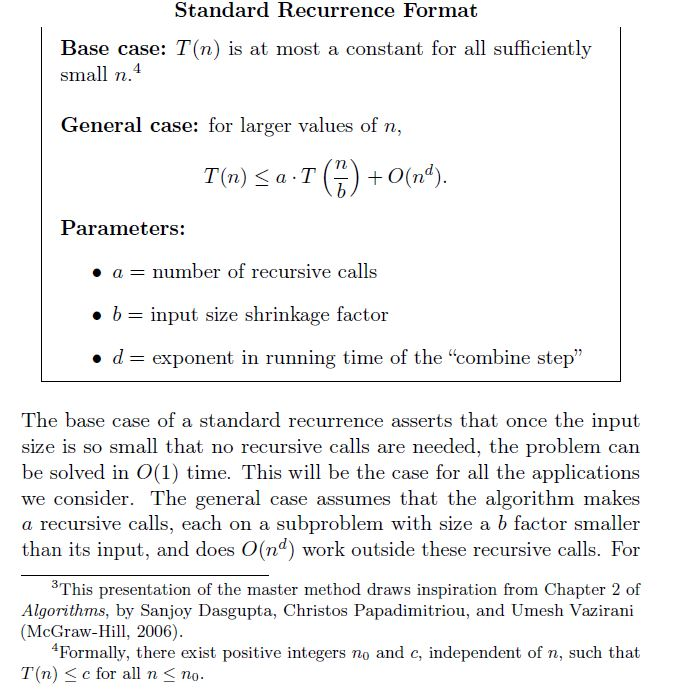
\includegraphics[scale = 0.5]{SRF}\\
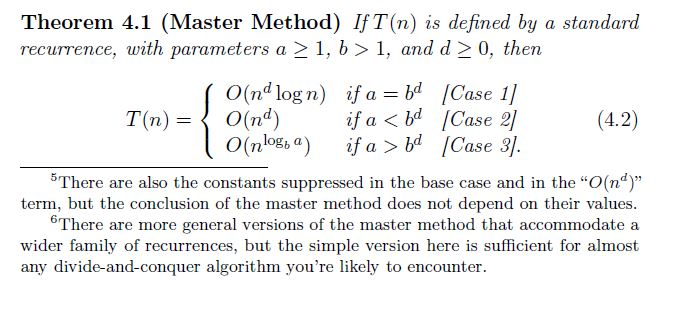
\includegraphics[scale = 0.5]{mm}\\
By the Master's Method I obtain $a = 2$, $b = 4$, $d = 0$ which gives us Case 3 since $a > b^d$. This gives me $O(n^{\log_4{2}}) = O(\sqrt{n})$. I have seen in other books make a stronger statement, saying that the function is $\Theta$ not $O$ with the master method but I trust Roughgarden more than the other sources I've found. Roughgarden has a good course on youtube in algorithmic game theory that I've taken notes from and has been teaching at Stanford and Coursera for many years.\\\\
Let us now attempt to prove, by induction, that $g(n) \epsilon \Theta(\sqrt{n})$. Let us assume that $g(n) = 16\sqrt{n} + \sqrt{n - 1} + 1$.\\\\\\\\\\\\\\\\
\textbf{Base Case}
\begin{align*}
g(1) &= 16\sqrt{1} + \sqrt{1 - 1} + 1\\
g(1) &= 16 + 0 + 1\\
g(1) &= 17\\
g(1) &= C\\
\end{align*}
For the case of argument, I don't know whether $C=17$. No domain was given for $C$ but it would seem plausible to me that the base case has been satisfied.\\\\
\textbf{Inductive Hypothesis}
\begin{align*}
T(n) &= 2^{1}T(\frac{n}{4^{1}}) + 16\\
T(n) &= 2^{2}T(\frac{n}{4^{2}}) + 16\\
T(n) &= 2^{3}T(\frac{n}{4^{3}}) + 16\\
T(n) &= 2^{4}T(\frac{n}{4^{4}}) + 16\\
&\vdots\\
T(n) &= 2^{\nabla}T(1) + 16\\
g(n) &= 16\sqrt{n} + \sqrt{n - 1} + 1\\
g(n) &\epsilon \Theta(\sqrt{n})\\
\end{align*}
\textbf{Inductive Step}
\begin{align*}
T(n + 1) &= 2^{\nabla+1}T(0) + 16\\
T(n + 1) &= 2(16\sqrt{n}) + 16\\
T(n + 1) &= 32\sqrt{n} + 16\\
\lim_{n\to\infty}{\frac{32\sqrt{n} + 16}{\sqrt{n}}} &\to32\\
&\therefore g(n)\epsilon \Theta(\sqrt{n})\\
\end{align*}\\
The series above was generated using mathematica and is an example of a puiseaux series. I don't like dealing with roots and I especially don't like taking limits of them so when I can I use mathematica to perform tranformations of them to a more usuable form. I believe by the nature of asymptotics I've answered the next two questions. This isn't how it was done in class, you proved both seperately but I look my notes and they're confusing.\\\\
I included simplifying of the root in fear of losing points due to not showing my work, but I used the series originally to solve the problem.\\  
\item [(5 points) 2.] State and prove by induction a theorem showing $T (n) \in O(g(n))$.

\item [(5 points) 3.] State and prove by induction a theorem showing $T (n) \in \Omega(g(n))$.
\end{enumerate}
\[
T(n) = \left\{
\begin{array}{cl}
c & \textrm{ if } n = 1\\
T(\left\lfloor\frac{n}{2}\right\rfloor) + T(\left\lfloor\frac{n}{4}\right\rfloor) + 4n & \textrm{ if } n > 1
\end{array}
\right.
\]
\\Before I present my recursion tree, let me for the sake of argument, state my assumptions: $2T(\frac{n}{4})+4n \leq T(\left\lfloor\frac{n}{2}\right\rfloor) + T(\left\lfloor\frac{n}{4}\right\rfloor) + 4n \leq 2T(\frac{n}{2})+4n$ since it is safe to assume that $T(n/4) \ll T(n/2)$. By the master method I expect that $g(n)$ should be sandwhiched in the following way $O(n) \ll g(n) \ll O(n\log{n})$\\
\begin{enumerate}
\item [(5 points) 1.] Draw the first six levels of the recursion tree by drawing all recursive calls of the same size on the same level. Make sure on each level you indicate the size of the recursive call and the number of recursive calls. \\\\
The recursion tree is in an attached document, labeled "recursiontree.pdf". I did not include that in this document because I could not get the LaTeX to format properly.\\\\
I'll state the levels here as joining them to the image is a lot of work.\\
Level 0: $4n$\\
Level 1: $4(\frac{n}{2^1}+\frac{n}{2^2})=3n$\\
Level 2: $4(\frac{n}{2^2}+\frac{n}{2^3}+\frac{n}{2^3}+\frac{n}{2^4})=\frac{9n}{4}$\\
For now on I will just state the sum result. The expressions became quite long and tedious.\\
Level 3: $\frac{27n}{16}$\\
Level 4: $\frac{81n}{64}$\\
Level 5: $\frac{243n}{256}$\\
Level 6: $\frac{729n}{1024}$\\
I thought I was doing something wrong but asside from algebra errors, I did follow pages 99-105 of Introduction to Algorithms (CLRS) to obtain this solution.\\\\
Apparently a property of each level being the same is only true if you have a single type of recurrence in an equation. If this had been for instance just $T(\frac{n}{4}) + n$ then you would have had equal costing levels at each recursion. You do not with this example.\\\\
According to the master method, I should expect the number of leaves ($L$) to be somewhere sandwhiched between $\sqrt{n} < L < n$ where $n$ is the number of nodes.\\
\item [(5 points) 2.] Express the cost of all levels of the recursion tree as a sum over the cost of each level of the recursion tree.\\\\
Looking back at the last page, there's clearly a linear recurrance of that. Solving for a linear recurrence can be quite difficult, so what is it that I expect the recurrance to be? I expect the recurrence to be some expression containing $\frac{1}{2}+\frac{1}{4}=\frac{2}{4}+\frac{1}{4}=\frac{3}{4}$. That appears to indeed be the case. To solve for the overall cost I will make the assumption that this tree is geometric and follow the examples from CLRS, knowing what I know from the above linear recurrence.\\
\item [(5 points) 3.] Give a function $g (n)$ and show it is an upper bound on the sum.
\begin{align*}
T(n) &\leq 4n + (\frac{3}{4})^1n+(\frac{3}{4})^2n+(\frac{3}{4})^3n+(\frac{3}{4})^4n+\dots\\
T(n) &\leq 3n + (\frac{3}{4})^0n + (\frac{3}{4})^1n+(\frac{3}{4})^2n+(\frac{3}{4})^3n+(\frac{3}{4})^4n+\dots\\
T(n) &\leq 3n + \sum_{\psi=0}^{\infty}{n(\frac{3}{4})^\psi}\\
T(n) &\leq 3n + \frac{n}{1-\frac{3}{4}}\\
T(n) &\leq 3n + 4n\\
T(n) &\leq 7n\\
T(n) &\epsilon O(n)
\end{align*}
This is a good upper bound but to find the exact bound I found the Akra-Bazzi method to be much more powerful, being as it seems well suited for such problems. I know that this value obtained must be smaller than the actual function for $g(n)$ because it is a geometric series that goes to infinity. The actual geometric series for this function would be finite in nature.\\\\
First we need to solve the equation $(\frac{1}{2})^p+(\frac{1}{4})^p=1$ obtaining $p=0.6942419136306174$.\\
\begin{align*}
T(n) &\epsilon \Theta(x^p(1+\int_{1}^{n}{u^{-p}du}))\\
T(n) &\epsilon \Theta(-2.27056n^{0.694242}+3.27056n)\\
T(n) &\epsilon \Theta(n)
\end{align*}\\
Not only is the other term lower in order but it is negative! We can safely ignore it. Akra-Bazzi seems powerful in that it can be shown that all recurrences can be shown to default to the non-recurrance term if $p$ is greater than the power of that polynomial term quickly simplifying the work needed to be done to find the asymptotic boundaries. I learned of this method from watching Lecture 14 in MIT 6.02J Mathematics for Computer Science Fall of 2018 timestamp $1:02:45$\\
\item [(5 points) 4.] State and prove by induction a theorem showing $T (n) \in O(g(n))$.
\item [(5 points) 5.] State and prove by induction a theorem showing $T (n) \in \Omega(g(n))$.\\\\
Let us assume that $T(n) \epsilon \Theta(n)$ where $g(n)=-2.27056n^{0.694242}+3.27056n$.\\\\
\[
T(n) = \left\{
\begin{array}{cl}
c & \textrm{ if } n = 1\\
T(\left\lfloor\frac{n}{2}\right\rfloor) + T(\left\lfloor\frac{n}{4}\right\rfloor) + 4n & \textrm{ if } n > 1
\end{array}
\right.
\]
\textbf{Base Case}\\
\begin{align*}
T(1) &= C\\
T(1) &= -2.27056(1)^{0.694242}+3.27056(1)\\
T(1) &= -2.27056+3.27056\\
T(1) &= 1\\
\end{align*}\\
Again no domain or value was given for $C$ but assuming that $C=1$ we can safely assume that the base case was satisfied.\\
\textbf{Inductive Hypothesis}\\
\begin{align*}
T(n) &=2^{\nabla}T(1) + 0 + 4n\\
g(n) &= -2.27056n^{0.694242}+3.27056n\forall{n>1}\\
g(n) &\epsilon \Theta(n)\\
\end{align*}\\
\textbf{Inductive Step}\\
If we look at our tree in the adjacent pdf, the leaves do not terminate in a uniform manner. This makes the problem illsuited for induction, but alas we will try.\\
\begin{align*}
T(n + 1) &=2^{\nabla + 1}T(0) + 0 + 4(n + 1)\\
T(n + 1) &=2(2^{\log{n}}T(1)) + 4n + 4\\
T(n + 1) &=2(n*1) + 4n + 4\\
T(n + 1) &=6n + 4\\
T(n+1) &\epsilon \Theta(n)\
\end{align*}\\
\\To assess my work let's recap. I've shown now that $3.27056n\leq g(n)\leq 6n<7n$. Clearly it is a function of $n$ and grows linearly. From Akra-Bazzi I know that if $p < $ power of the additional term, which in this case is true, $0.6942419136306174 < 1$ then we know that the $n$ term will dominate in the expression for $T(n)$. The reccurence terms fall away for large n. 
\end{enumerate}
\end{enumerate}
\end{document}